\subsection{ Naive Bayes }

First experiment is using naive bayes classifier to find, the probability of being a word is `keyword' or `not'. We tokenized the text into sentences and words. Term frequency and Inverse Document Frequency is calculated after stemming the words.  

\textit{titleScore} is the probability of word being generated from title text. Often cases, title words are given importance, but difficulty is title is small in size so most of the cases the acronyms or shortened word. For example \textit{united states} in text corresponds to \textit{U.S.} in title, \textit{mahindra singh doni} in text corresponds to \textit{mahi} in title. 

\textit{IDFTF} score calculated based IR approaches.\textit{Postag} for each word is obtained from Stanford PCFG parser.


Final score is calculated based on,

$
P(Key/Word, PosTag, IDFTF, titleScore) 
$
\begin{align}
= P(Key) * P(Word/Key) * P(PosTag/Key) * P(IDFTF/Key) * P(titleScore/Key)
\end{align}

Graphical model digram of Naive bayes approach is depicted in ~\ref{fig:nbc}

\begin{figure}[H]
\begin{center}
\fbox{\scalebox{0.7}{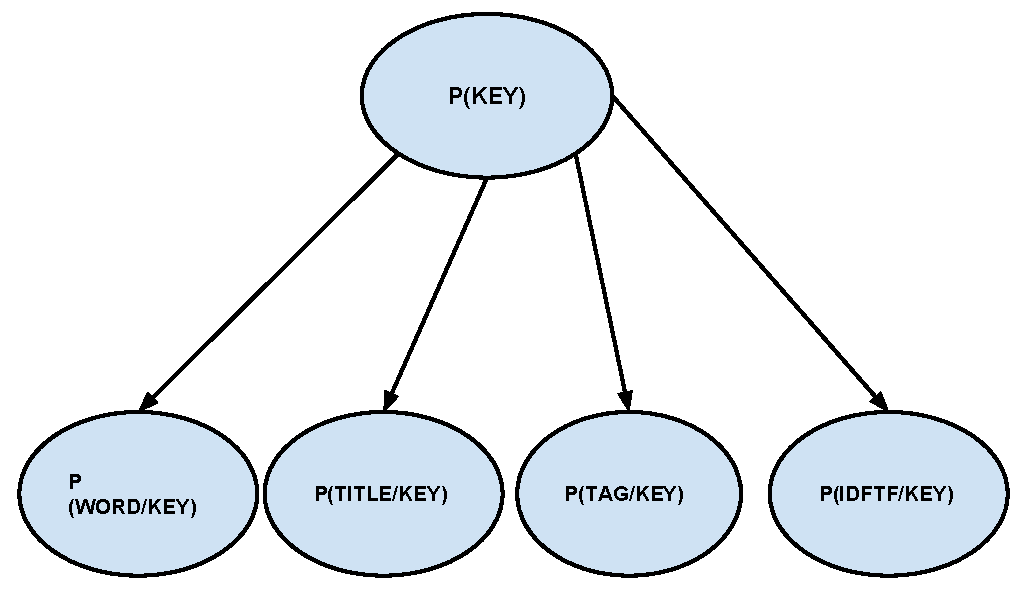
\includegraphics{nbc.pdf}}}
\end{center}
\caption{Naive Bayes Classification}
\label{fig:nbc}
\end{figure}

We tested this method with 50 articles, its title and meta data extracted from Yahoo! News.
Keywords extracted using this system achieves  20\% overlap on metadata text. 
%\textbf{Results:}\todosmall{TODO}